\documentclass{article}
\usepackage[utf8]{inputenc}
\usepackage[margin= .8in]{geometry}
\usepackage{graphicx}
\usepackage{float}

\title{Interference pattern obtained from \\ two free particle quantum systems in superposition}
\author{Daniel Hern�ndez Mota }
\date{Spring 2019}

\begin{document}

\maketitle

\section{Introduction}
Quantum Mechanics was born due to the intimacy of the development of experimental research. It is now well known that the properties of atomic and sub atomic systems differ widely from the macroscopic system's properties. This is the case for the free particle. Classically we can think of a free particle as a body with a mass $m$ at constant velocity, with no interaction of any potential. However, in quantum mechanics the free particle can carry any energy, nevertheless, there is no such thing as a free particle with a definite energy. Superpositions of wave packets lead to interference which allows localization and normalizability.

\section{Free Particle}
It is possible to obtain a general wave function from the Schr�dinger equation's solution of a free particle:

\begin{equation}
    \Psi = \left(2\pi \sigma^2\right)^{-1/4}\frac{\sigma}{\sqrt{\sigma^2+ \frac{i\hbar t}{2m\sigma}}}e^{-\frac{(x-x_0-2i\sigma^2k_0)^2}{4\sqrt{\sigma^2+ \frac{i\hbar t}{2m\sigma}}}-\sigma^2k_0^2+ik_0x}
\end{equation}

One can graph this function an position $x$ indicated for N points with a range from \textit{b} to \textit{a} and giving the necessary parameters $t$, $x_0$, $\sigma$, and $k_0$.

In this case, the general parameters were defined as following:

\begin{equation}
    x\in[a,b]=[-10,10];\quad N=1000
\end{equation}


\subsection{First wave-function}
By evaluating the function with the following parameters, a graph corresponding to the real and imaginary components can be created. 

\begin{equation}
    t=0;\quad x_0=0;\quad \sigma=1.5;\quad k_0 = 1.5
\end{equation}

\begin{figure}[H]
    \centering
    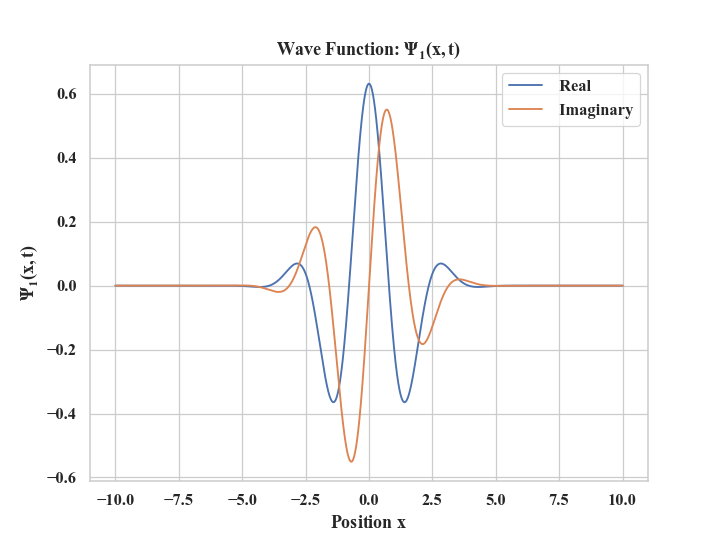
\includegraphics[scale=0.45]{Images/wave_func1.png}
    \caption{First wave-function: $\Psi_1$}
    \label{fig:wf1}
\end{figure}

\subsection{Second wave-function}
By evaluating the function with similar parameters, another graph can be generated.

\begin{equation}
    t=0;\quad x_0=0;\quad \sigma=2.0;\quad k_0 = 6.0
\end{equation}

\begin{figure}[H]
    \centering
    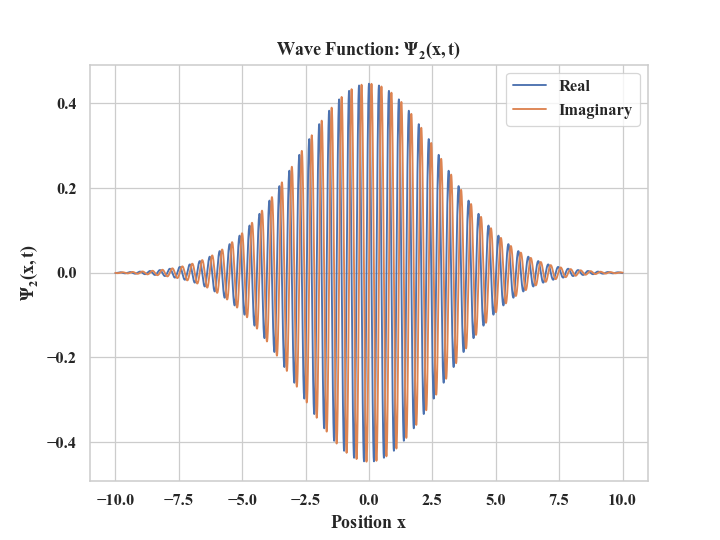
\includegraphics[scale=0.45]{Images/wave_func2.png}
    \caption{Wave-function: $\Psi_2$}
    \label{fig:wf2}
\end{figure}

\subsection{Superposition}
Given that two wave-functions can be in a superposition state, it is possible to obtain a third wave-function that is a linear combination of the last two.

To do this, a new wave-function can be created with the condition of re-normalization. 

\begin{equation}
    \Psi_3 = \frac{1}{\sqrt{2}}\left(\Psi_1-\Psi_2\right)
\end{equation}

\begin{figure}[H]
    \centering
    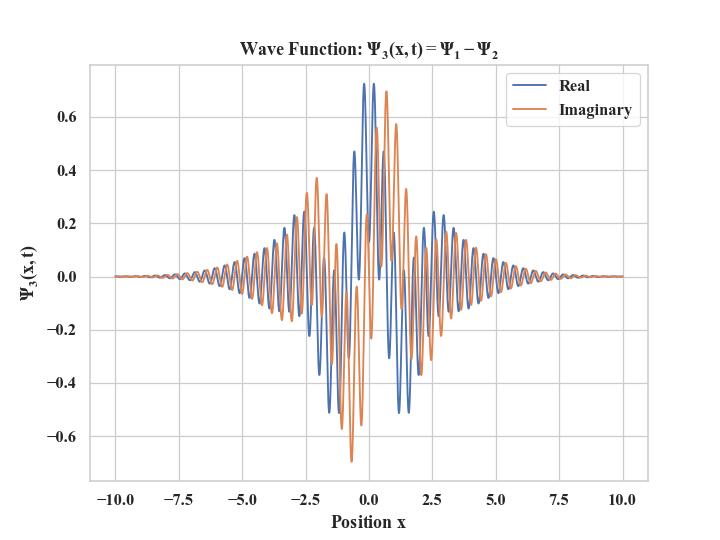
\includegraphics[scale=0.45]{Images/wave_func3.png}
    \caption{Wave-function: $\Psi_37$}
    \label{fig:wf3}
\end{figure}

\section{Probabilities}

To determine the probability to find a particle in this state, the squared magnitude of the wave-function can be obtained, this actually yields a probability density function

\begin{figure}[H]
    \centering
    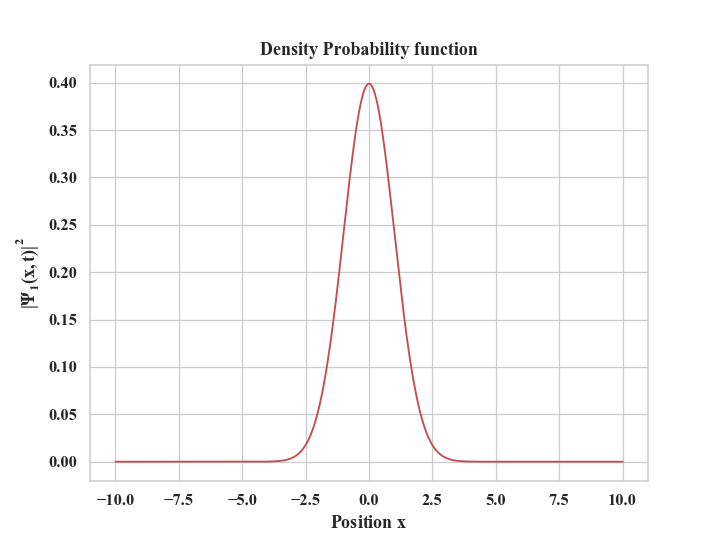
\includegraphics[scale=0.45]{Images/prob_1.png}
    \caption{Probability of the first wave-function, $\Psi_1$}
    \label{fig:prob_1}
\end{figure}

\begin{figure}[H]
    \centering
    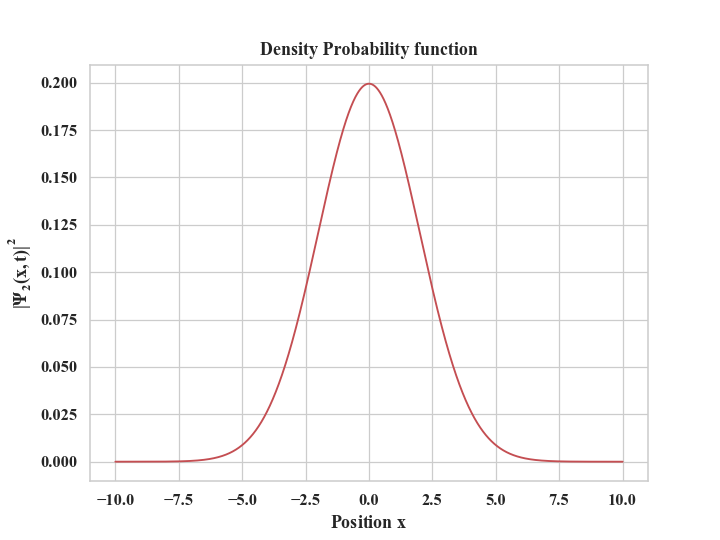
\includegraphics[scale=0.45]{Images/prob_2.png}
    \caption{Probability of the second wave-function, $\Psi_2$}
    \label{fig:prob_2}
\end{figure}


In some cases, it is possible to find an interference pattern in the probabilities due to the superposition of different quantum states:

\begin{figure}[H]
    \centering
    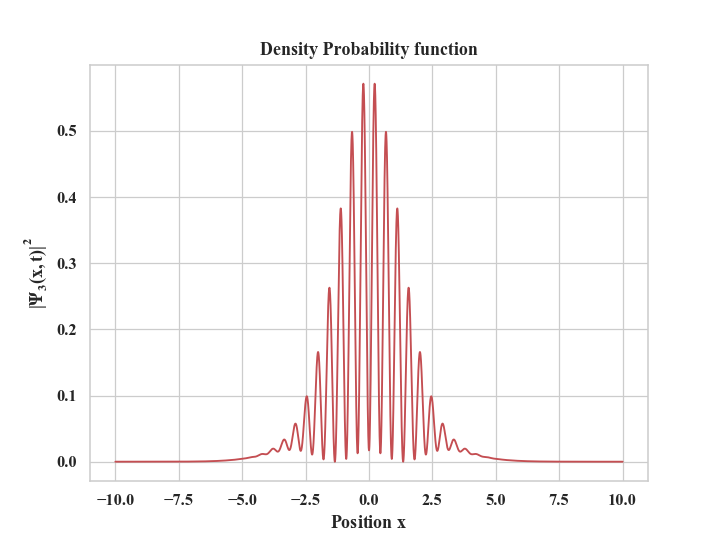
\includegraphics[scale=0.45]{Images/prob_3.png}
    \caption{Probability of the third wave-function, $\Psi_3$}
    \label{fig:prob_3}
\end{figure}

\section{Experiment}

Considering the probability density function of the third wave-function, an experiment can be realized.

\begin{figure}[H]
    \centering
    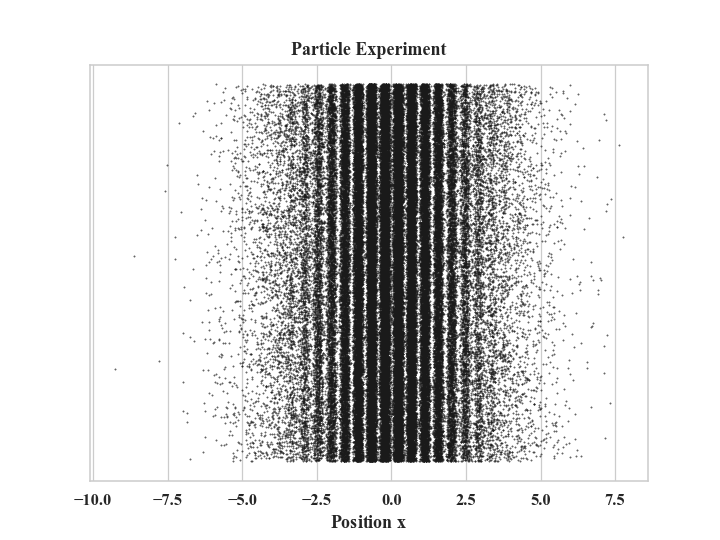
\includegraphics[scale=0.45]{Images/exp.png}
    \caption{Experiment}
    \label{fig:exp}
\end{figure}

The behavior of the particles can be tested by overlapping the probability density function with the results.

\begin{figure}[H]
    \centering
    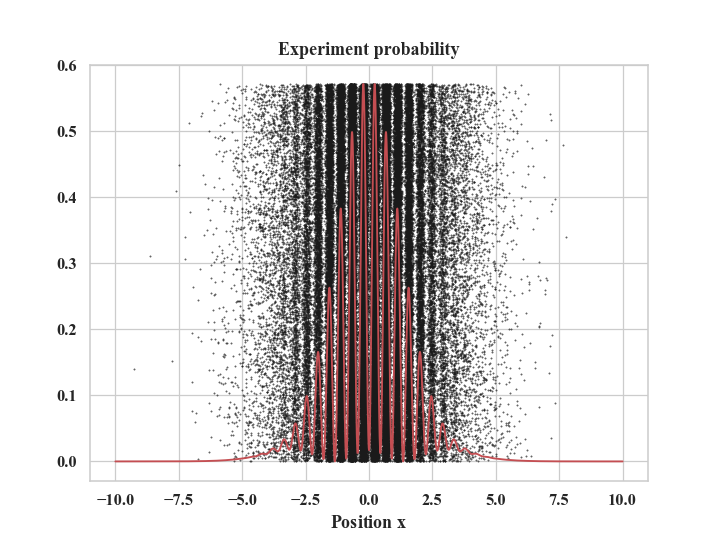
\includegraphics[scale=0.45]{Images/over.png}
    \caption{Experiment and overlapping of the probability density function}
    \label{fig:ovelap}
\end{figure}

\end{document}